\chapter{Control System Implementation}
\label{implementation_of_controller}

This chapter will explain how the controller designed in \chapref{Controller} is implemented on the scaled system at Aalborg university.  

\section{Simulink implementation}
\label{simulink_intro}
In the implementation of the control, the model estimated in \secref{estim_results} is used. Although, the fit percentage differs from the real data, the behavior and dynamics of the WT are correctly caught, making this model the most suitable and realistic to work with. \figref{fig:control_sketch} shows the implementation strategy for the control design on the model of the water distribution system.
% It is worth mentioning, that for the implementation of the control, the second linear model attempt is used as it is the most suitable model to work with. The MPC controller is implemented in MATLAB Simulink, which is connected to the model as shown in \figref{fig:control_sketch}:

\begin{figure}[H]
\centering
\input{report/tikz/Control_Layout.tex} 
\caption{Sketch of the control implementation.}
\label{fig:control_sketch}
\end{figure}

From the state-space model, the WT pressure is sent to the MPC block at each iteration, as the current initial state is measured and required for calculating the constraints and the objective function. 

In order to solve the optimization problem and find a global minimum for the problem specified in \eqref{eq:obj_final1},  Quadratic Programming(QP) is used. Solvers for QP problems in Matlab find out the preceding problem subject to the specified constraints and restrictions set to the convex function. The method chosen is interior-point-convex algorithm which solves the problem by simplifying the constraints and then by iterating in the interior of the feasible set.  Progressively, it adds the constraints and reconstructs the original problem \cite{Convex_optimization}. 

In previous sections, the length of the prediction horizon, $H_p$, is introduced. It is decided to predict 24 hour forward due to the periodicity of the electricity price and the behavior of the end-user consumption. Therefore, the control input to the state-space model and the disturbance due to the end-users are updated every hour. The sampling time for the control input will differ from the sample time determined for the discrete time state-space model, which is $T_s = 87.5s$. 

In \appref{sec:cost_fkt}, the electric price model is shown. Nevertheless, for the implementation of the control not only the electric price model is needed but also a model for the end-user water consumption. This can be seen in \figref{fig:water_consumption}

\begin{figure}[H]
\centering
% This file was created by matlab2tikz.
%
%The latest updates can be retrieved from
%  http://www.mathworks.com/matlabcentral/fileexchange/22022-matlab2tikz-matlab2tikz
%where you can also make suggestions and rate matlab2tikz.
%
\definecolor{mycolor1}{rgb}{0.00000,0.44700,0.74100}%
%
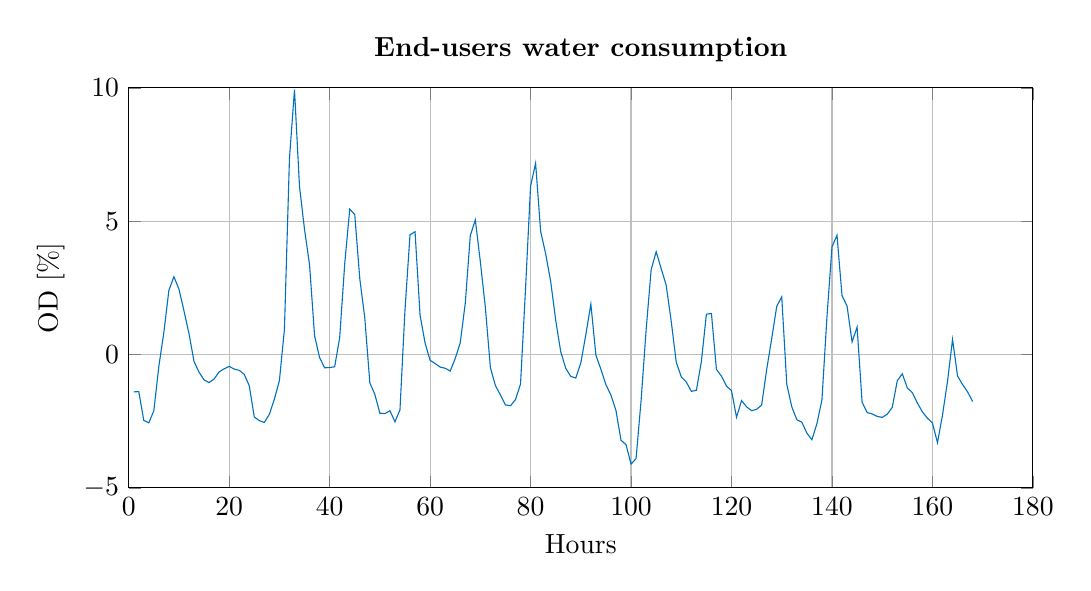
\begin{tikzpicture}

\begin{axis}[%
width=4.521in,
height=2in,
at={(1.011in,0.642in)},
scale only axis,
xmin=0,
xmax=180,
xlabel={Hours},
xmajorgrids,
ymin=-5,
ymax=10,
ylabel={OD [\%]},
ymajorgrids,
axis background/.style={fill=white},
title style={font=\bfseries},
title={End-users water consumption}
]
\addplot [color=mycolor1,solid,forget plot]
  table[row sep=crcr]{%
1	-1.40016249999999\\
2	-1.38966249999999\\
3	-2.46766249999999\\
4	-2.5611125\\
5	-2.1106625\\
6	-0.436962499999995\\
7	0.834237500000005\\
8	2.41203750000001\\
9	2.9167375\\
10	2.4533375\\
11	1.64133750000001\\
12	0.781737500000005\\
13	-0.259862499999995\\
14	-0.660262499999995\\
15	-0.952162499999994\\
16	-1.0508625\\
17	-0.915762499999995\\
18	-0.650462499999994\\
19	-0.535662499999995\\
20	-0.441862499999995\\
21	-0.546162499999995\\
22	-0.593062499999994\\
23	-0.744262499999994\\
24	-1.17091249999999\\
25	-2.3402625\\
26	-2.47851249999999\\
27	-2.54886249999999\\
28	-2.2387625\\
29	-1.67386249999999\\
30	-0.975962499999994\\
31	0.948337500000004\\
32	7.34633750000001\\
33	9.93003750000001\\
34	6.2998375\\
35	4.69053750000001\\
36	3.3675375\\
37	0.706137500000006\\
38	-0.116362499999994\\
39	-0.497162499999994\\
40	-0.486662499999996\\
41	-0.460062499999994\\
42	0.638237500000006\\
43	3.3990375\\
44	5.4556375\\
45	5.24773750000001\\
46	2.84673750000001\\
47	1.36763750000001\\
48	-1.05926249999999\\
49	-1.4974625\\
50	-2.2002625\\
51	-2.21636249999999\\
52	-2.10646249999999\\
53	-2.5236625\\
54	-2.0756625\\
55	1.6791375\\
56	4.49173750000001\\
57	4.6065375\\
58	1.47613750000001\\
59	0.429637500000005\\
60	-0.216462499999995\\
61	-0.336162499999995\\
62	-0.471262499999996\\
63	-0.513262499999995\\
64	-0.617562499999994\\
65	-0.148562499999995\\
66	0.440137500000005\\
67	1.9290375\\
68	4.46023750000001\\
69	5.0489375\\
70	3.4816375\\
71	1.76243750000001\\
72	-0.492262499999995\\
73	-1.16216249999999\\
74	-1.51636249999999\\
75	-1.8915625\\
76	-1.9174625\\
77	-1.68856249999999\\
78	-1.10546249999999\\
79	2.4883375\\
80	6.31663750000001\\
81	7.17623750000001\\
82	4.6240375\\
83	3.7801875\\
84	2.74383750000001\\
85	1.28818750000001\\
86	0.108337500000004\\
87	-0.516762499999994\\
88	-0.818812499999994\\
89	-0.881112499999995\\
90	-0.318662499999995\\
91	0.746387500000005\\
92	1.89473750000001\\
93	-0.0190624999999952\\
94	-0.553162499999995\\
95	-1.13136249999999\\
96	-1.5219625\\
97	-2.09806249999999\\
98	-3.2124625\\
99	-3.3790625\\
100	-4.1077625\\
101	-3.8998625\\
102	-1.72006249999999\\
103	0.914737500000005\\
104	3.17713750000001\\
105	3.85683750000001\\
106	3.22158750000001\\
107	2.5989375\\
108	1.24023750000001\\
109	-0.288212499999995\\
110	-0.835262499999995\\
111	-1.03021249999999\\
112	-1.3791625\\
113	-1.34276249999999\\
114	-0.264762499999995\\
115	1.51113750000001\\
116	1.54193750000001\\
117	-0.556662499999996\\
118	-0.811462499999995\\
119	-1.1866625\\
120	-1.3532625\\
121	-2.35146249999999\\
122	-1.7270625\\
123	-1.9608625\\
124	-2.10646249999999\\
125	-2.05466249999999\\
126	-1.8936625\\
127	-0.560862499999996\\
128	0.594837500000006\\
129	1.8079375\\
130	2.16213750000001\\
131	-1.1124625\\
132	-1.9608625\\
133	-2.4424625\\
134	-2.5390625\\
135	-2.94506249999999\\
136	-3.1949625\\
137	-2.5936625\\
138	-1.7032625\\
139	1.41243750000001\\
140	4.03603750000001\\
141	4.47353750000001\\
142	2.2090375\\
143	1.8233375\\
144	0.475137500000005\\
145	1.02743750000001\\
146	-1.79426249999999\\
147	-2.17436249999999\\
148	-2.2261625\\
149	-2.3199625\\
150	-2.35636249999999\\
151	-2.2366625\\
152	-1.9811625\\
153	-0.981562499999995\\
154	-0.721862499999995\\
155	-1.2524625\\
156	-1.4295625\\
157	-1.82016249999999\\
158	-2.1477625\\
159	-2.3878625\\
160	-2.56426249999999\\
161	-3.3090625\\
162	-2.27026249999999\\
163	-1.0029125\\
164	0.564037500000006\\
165	-0.805162499999995\\
166	-1.1278625\\
167	-1.39806249999999\\
168	-1.7627625\\
};
\end{axis}
\end{tikzpicture}% 
\caption{End-users water consumption, with acts as a disturbance to the system.}
\label{fig:water_consumption}
\end{figure}

In this case the model is created to last for a week and then repeats. 


\section{Simulink results}
The MPC problem set up to optimize the power consumption of the pumps, developed through \secref{sec:MPC}, has been proved to be convex, in \secref{convexity}. In this way, the main feature of this controller is the ability to reduce the cost of running the system based on the electric price and the WT level. 

After implementing the MPC, described in \secref{simulink_intro}, multiple complications occurred. The optimization problem is implemented with only the input constraints. This is done to check that the simpler optimization problem can be solved. The input constraints are added to guarantee that pumps do not run outside their physical limits. 

Since there are not any constraints applied to either the pressure at the WT or the CP, it is expected to see that the input signal is as low as possible the during operation. This behavior, compared to the real system, is expected because the cheapest way of running the pumps would be as slow as possible. 

\begin{figure}[H]
\centering
% This file was created by matlab2tikz.
%
%The latest updates can be retrieved from
%  http://www.mathworks.com/matlabcentral/fileexchange/22022-matlab2tikz-matlab2tikz
%where you can also make suggestions and rate matlab2tikz.
%
\definecolor{mycolor1}{rgb}{0.00000,0.44700,0.74100}%
%
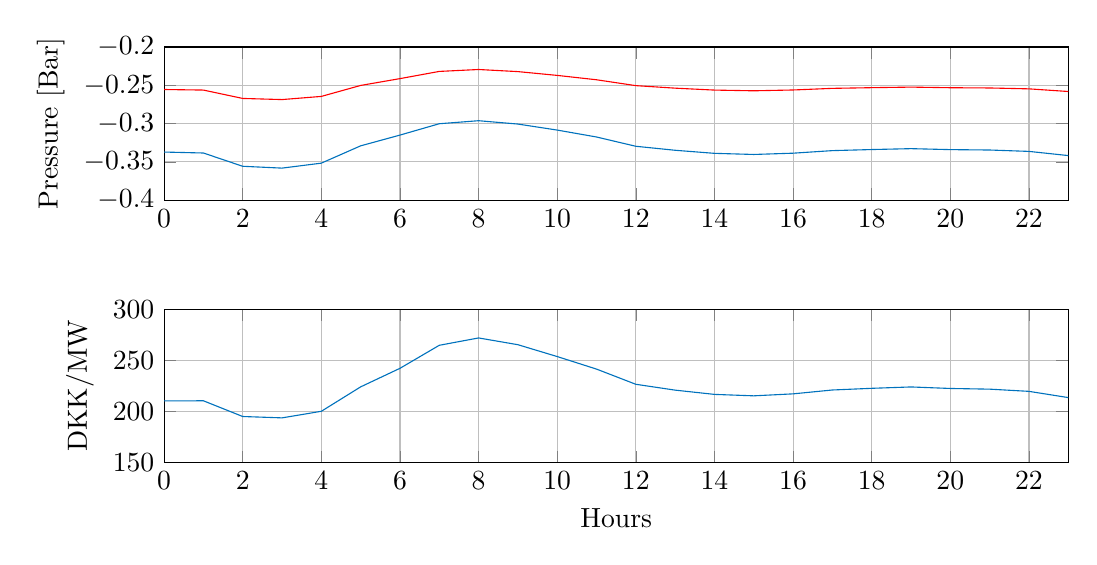
\begin{tikzpicture}

\begin{axis}[%
width=4.521in,
height=0.766in,
at={(0.758in,3.103in)},
scale only axis,
xmin=0,
xmax=23,
xmajorgrids,
ymin=-0.4,
ymax=-0.2,
ymajorgrids,
ylabel={Pressure [Bar]},
axis background/.style={fill=white}
]
\addplot [color=mycolor1,solid,forget plot]
  table[row sep=crcr]{%
0	-0.337187128298502\\
1	-0.338428175857978\\
2	-0.355759379672392\\
3	-0.358161526141837\\
4	-0.351679783260157\\
5	-0.329079947578111\\
6	-0.315052123868196\\
7	-0.30021579160496\\
8	-0.296274053706477\\
9	-0.300647937847971\\
10	-0.308494586422369\\
11	-0.317532459852742\\
12	-0.329652163199425\\
13	-0.334869915814744\\
14	-0.338864209741175\\
15	-0.340341790313779\\
16	-0.338670164645983\\
17	-0.335322051533021\\
18	-0.333915730131158\\
19	-0.332752769322142\\
20	-0.334012136632997\\
21	-0.334527251444417\\
22	-0.33633206106221\\
23	-0.341786804661069\\
};

\addplot [color=red,solid,forget plot]
  table[row sep=crcr]{%
0	-0.255539239876202\\
1	-0.25626975504531\\
2	-0.26719592758736\\
3	-0.268681742866465\\
4	-0.264551418136899\\
5	-0.250228419704096\\
6	-0.241331839560681\\
7	-0.231926715572023\\
8	-0.229416388743334\\
9	-0.232168715735042\\
10	-0.237119565456248\\
11	-0.242825434953476\\
12	-0.250482475520783\\
13	-0.253774199452117\\
14	-0.256293452004186\\
15	-0.257221941508702\\
16	-0.256159380174046\\
17	-0.254037538765411\\
18	-0.253146005750368\\
19	-0.252409936615807\\
20	-0.253208396629209\\
21	-0.253537295911981\\
22	-0.254684115730977\\
23	-0.258143242409582\\
};
\end{axis}

\begin{axis}[%
width=4.521in,
height=0.766in,
at={(0.758in,1.792in)},
scale only axis,
xmin=0,
xmax=23,
xmajorgrids,
xlabel={Hours},
ymin=150,
ymax=300,
ymajorgrids,
ylabel={DKK/MW},
axis background/.style={fill=white}
]
\addplot [color=mycolor1,solid,forget plot]
  table[row sep=crcr]{%
0	210.15\\
1	210.3\\
2	194.9\\
3	193.565\\
4	200\\
5	223.91\\
6	242.07\\
7	264.61\\
8	271.82\\
9	265.2\\
10	253.6\\
11	241.32\\
12	226.44\\
13	220.72\\
14	216.55\\
15	215.14\\
16	217.07\\
17	220.86\\
18	222.5\\
19	223.84\\
20	222.35\\
21	221.68\\
22	219.52\\
23	213.425\\
};
\end{axis}
\end{tikzpicture}% 
\caption{Implemented optimizer, without constraints. The first figure show the two pumps, pump one can be seen in red and pump two as blue. The second figure shows the cost of electricity for the first 24 hours.}
\label{fig:Implementation_shit}
\end{figure}

In \figref{fig:Implementation_shit} the electrical price and both input signal to the pumps can be seen. Here it can be seen that the input to the first pump is constant at $0.05$ and $0.03$, the lower bounds for the pumps respectively. If an input signal lower then this is applied to the pumps they will start acting unstable. 

The remaining constraints, consisting of the pressure at the WT and the CP, are added and consequently no infeasible solution is found. This is also the case when only one of the constraint is added. 

This could occur because the model, used in the implementation is simplification of the real world. In order to set up the constraints for the optimizing problem, the physical limitations of the system setup have been determined. These values are obtained under the operating point conditions of the system, so that they remain under reasonable regions for the linearized model. Nevertheless, these values would be feasible for the estimated model if and only if the model had represented the real setup perfectly. As described in \secref{estim_results} the estimation has been carried out so the dynamics of the WT are prioritized rather than obtaining a closer fit percentage for the model. Therefore, the physical limits calculated for the real setup cannot be utilized for the simulation model, making the quadratic problem to be infeasible within the specified constraints. This infeasibility means that not all constraints can be satisfied at a single solution $\bm{u}$.

The optimizing problem design is hereby finished as the MPC control has been implemented together with the estimated model. On the one hand, it is shown that the unconstrained problem is solvable and expected values are obtained. On the other hand, the problem cannot be completed due to the incapability to calculate a control input once the constraints of the system are set. Any further discussion on the subject is brought up in the following chapter. 

%\subsection{Summary of implementation}
%The MPC, from \chapref{Controller}, is tried implemented and seems to be work at first. 


%seemed to be infeasible. As a results of this no minimum was found. MUltiple attempts to solve this problem was done and 

%
% vis at vores optimering virker når vi kun bruger lb og ub. Dog kan det ses at intputet stiger når prisen stiger, hvilket kunne tyde på en fortegnsfejl
%
% Når vi tilføjer flere constrints går det helt galt og problemet er infeasible  
%
%
%
